
\begin{frame}
\frametitle{Generative models for classification}
\begin{columns}[c]
\column{0.5\textwidth}
\begin{align*}
P(y\!=\!k|{\bf x}) = \frac{P(y\!=\!k) p({\bf x}|y\!=\!k)}{\sum_j P(y\!=\!j) p({\bf x}|y\!=\!j)}
\end{align*}
\column{0.5\textwidth}
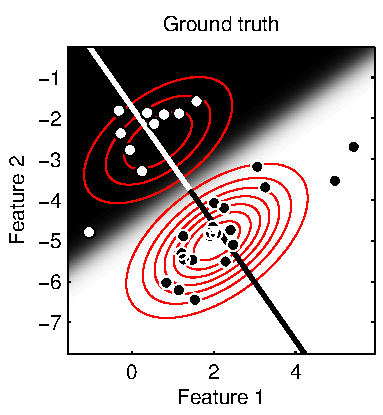
\includegraphics[width=\textwidth]{simple_ground_truth}
\end{columns}
\end{frame}

\begin{frame}
\frametitle{Linear discriminant analysis}
\begin{columns}[c]
\column{0.5\textwidth}
\begin{align*}
P(y\!=\!k|{\bf x}) = \frac{P(y\!=\!k) p({\bf x}|y\!=\!k)}{\sum_j P(y\!=\!j) p({\bf x}|y\!=\!j)}
\end{align*}
Assumes:
\begin{align*}
P({\bf x}|y\!=\!k) = \mathcal{N}({\bf x} | {\boldsymbol\mu}_k, \boldsymbol\Sigma)
\end{align*}
\column{0.5\textwidth}
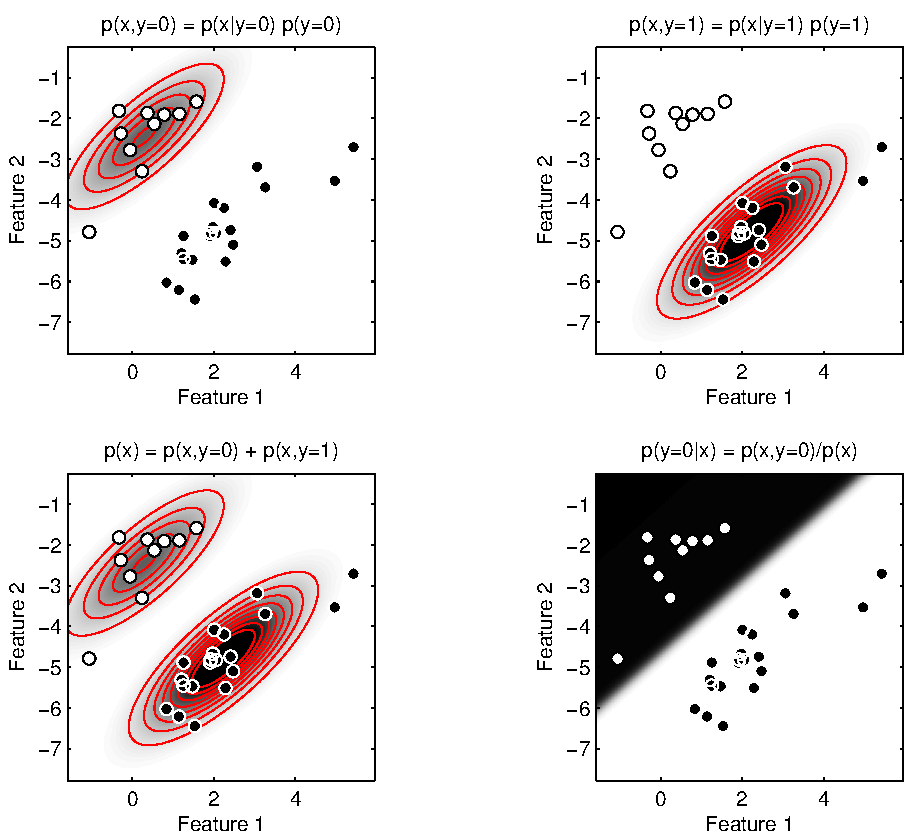
\includegraphics[width=\textwidth]{simple_fld}
\end{columns}
Model has $2p + p(p-1)$ parameters to estimate (two means and a single covariance).\par
Number of observations is $pn$ (size of inputs).
\end{frame}

\begin{frame}
\frametitle{Quadratic discriminant analysis}
\begin{columns}[c]
\column{0.5\textwidth}
\begin{align*}
P(y\!=\!k|{\bf x}) = \frac{P(y\!=\!k) p({\bf x}|y\!=\!k)}{\sum_j P(y\!=\!j) p({\bf x}|y\!=\!j)}
\end{align*}
Assumes different covariances:
\begin{align*}
P({\bf x}|y\!=\!k) = \mathcal{N}({\bf x} | {\boldsymbol\mu}_k, {\boldsymbol\Sigma}_k)
\end{align*}
\column{0.5\textwidth}
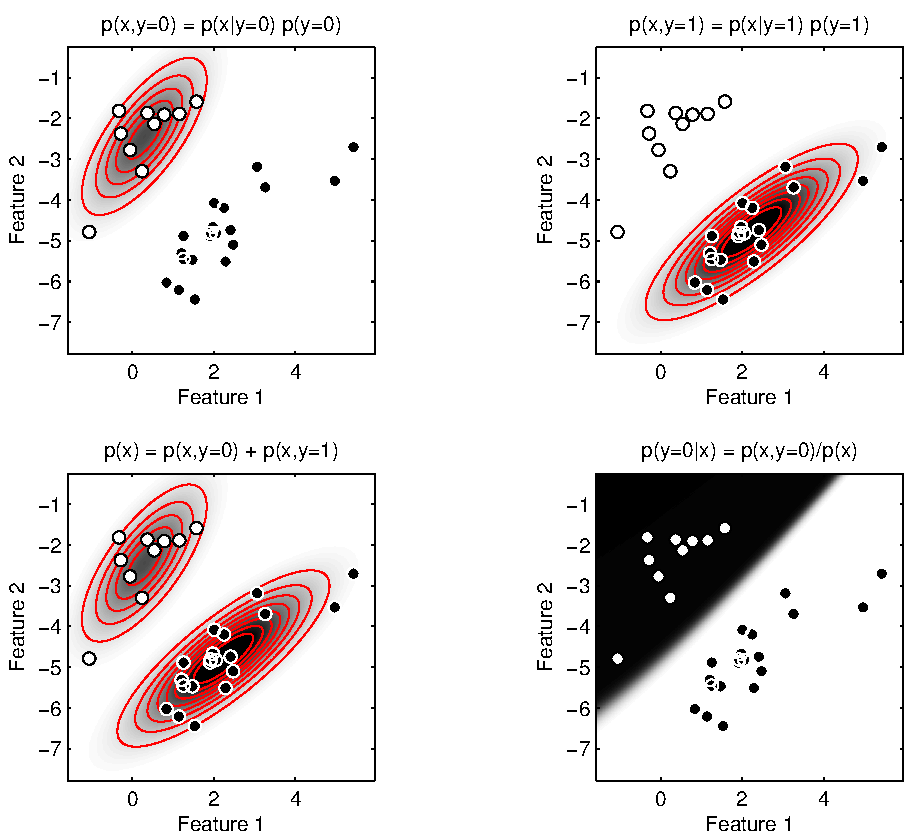
\includegraphics[width=\textwidth]{simple_qda}
\end{columns}
Model has $2p + 2p(p-1)$ parameters to estimate (two means and two covariances).\par
Number of observations is $pn$.
\end{frame}

\begin{frame}
\frametitle{Naive Bayes}
\begin{columns}[c]
\column{0.5\textwidth}
\begin{align*}
P(y\!=\!k|{\bf x}) = \frac{P(y\!=\!k) p({\bf x}|y\!=\!k)}{\sum_j P(y\!=\!j) p({\bf x}|y\!=\!j)}\cr
\end{align*}
Assumes that features are independent:
\begin{align*}
p({\bf x}|y\!=\!k) = \prod_i p(x_i|y\!=\!k)
\end{align*}
\column{0.5\textwidth}
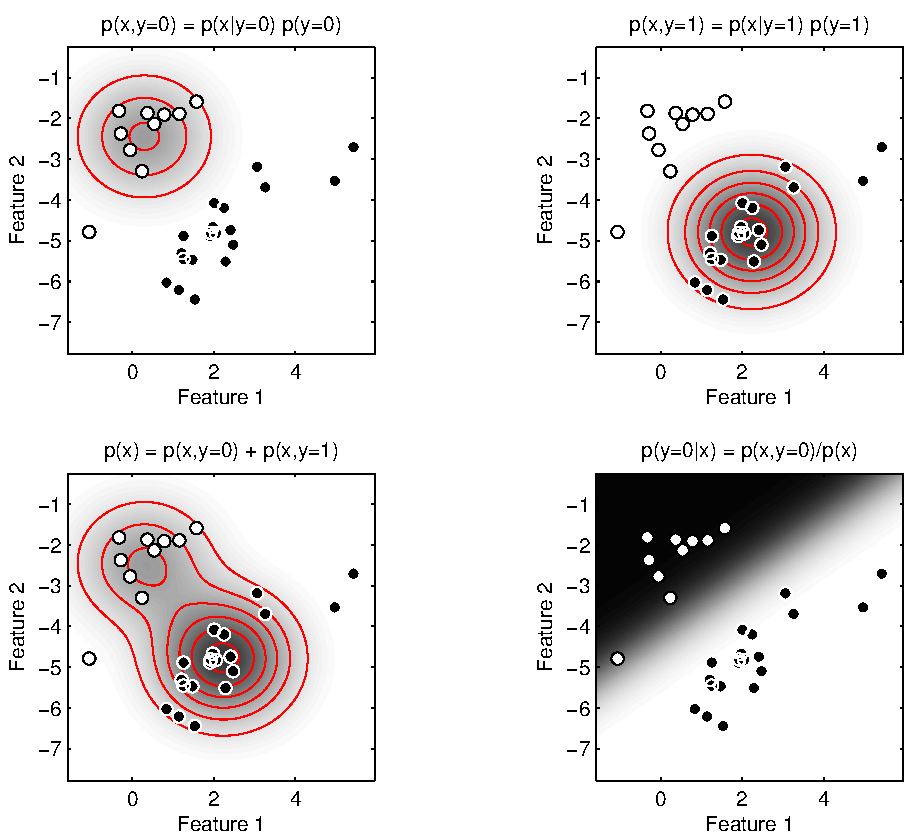
\includegraphics[width=\textwidth]{simple_naive_bayes}
\end{columns}
Model has variable number of parameters to estimate, but the above example has $3p$.\par
Number of observations is $pn$.
\end{frame}

\begin{frame}
\frametitle{Linear regression: maximum likelihood}
\begin{align*}
f({\bf x}_*) = {\bf a}^T {\bf x}_*
\end{align*}
Assuming Gaussian noise on ${\bf y}$, the ML estimate of ${\bf a}$ is by:
\begin{align*}
\hat{\bf a} = ({\bf X}{\bf X}^T)^{-1}{\bf X} {\bf y}
\end{align*}
where
\begin{align*}
{\bf X} = \begin{pmatrix}{\bf x}_1 & {\bf x}_2 & \hdots & {\bf x}_n\end{pmatrix}^T \text{, and }
{\bf y} = \begin{pmatrix}y_1 & y_2 & \hdots y_n\end{pmatrix}^T
\end{align*}
Model has $p$ parameters to estimate.\par
Number of observations is $n$ (number of targets).
\end{frame}

\begin{frame}
\frametitle{Linear regression: maximum posterior}
\begin{align*}
y \sim & \mathcal{N}({\bf a}^T {\bf x},\sigma^2)\\
{\bf a} \sim & \mathcal{N}({\bf 0},\Sigma_0)
\end{align*}
Maximum a posteriori (MAP) estimate of ${\bf a}$ is by:
\begin{align*}
\hat{\bf a} = \sigma^{-2}{\bf C}^{-1}{\bf X}{\bf y} \text{, where } {\bf C} = \sigma^{-2}{\bf X}{\bf X}^T + \Sigma_0^{-1}
\end{align*}
Number of estimated parameters and observations is ill defined.
\end{frame}

\begin{frame}
\frametitle{Linear regression: Bayesian}
\begin{align*}
p(y_* | {\bf x}_*, {\bf a}) = & \mathcal{N}({\bf a}^T{\bf x}_*, \sigma^2)\cr
p({\bf a}|{\bf y},{\bf X})  = & \mathcal{N}(\sigma^{-2}{\bf C}^{-1}{\bf X}{\bf y},{\bf C}^{-1}) \text{, where } {\bf C} = \sigma^{-2}{\bf X}{\bf X}^T + \Sigma_0^{-1}
\end{align*}
\begin{align*}
p(y_* | {\bf x}_*, {\bf y}, {\bf X}) = & \int_{\bf a} p(y_* | {\bf x}_*, {\bf a}) p({\bf a}|{\bf y},{\bf X}) d{\bf a}\cr
                                     = & \mathcal{N}(\sigma^{-2} {\bf x}_*^T {\bf C}^{-1} {\bf X} {\bf y}, {\bf x}_*^T{\bf C}^{-1}{\bf x}_*)
\end{align*}
Weights are integrated out - rather than estimated.\par
Estimated parameters may be $\sigma^2$, and parameters encoding $\Sigma_0$.
\end{frame}


\begin{frame}
\frametitle{Discriminative models for classification}
\begin{columns}[c]
\column{0.5\textwidth}
\begin{align*}
t = f({\bf a}^T {\bf x})
\end{align*}
where $f$ is some squashing function, eg:
\begin{itemize}
\item Heaviside step function.
\item Logistic function (inverse of Logit).
\item Normal CDF (inverse of Probit).
\end{itemize}
\column{0.5\textwidth}
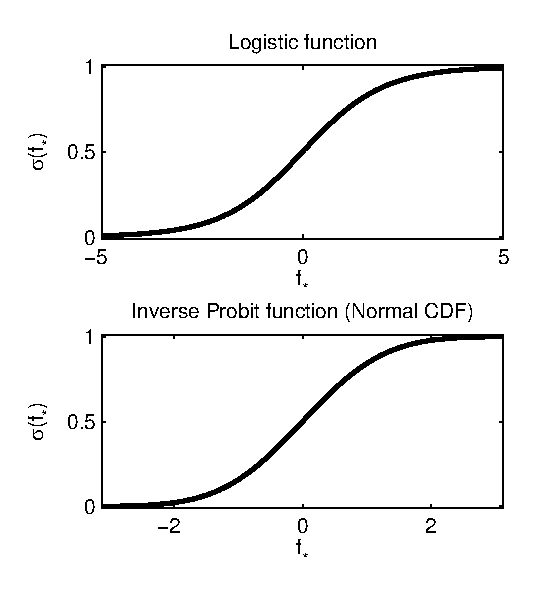
\includegraphics[width=.75\textwidth]{squashing}
\end{columns}
\end{frame}

\begin{frame}
\frametitle{Probabilistic classification}
\begin{columns}[c]
\column{0.5\textwidth}
\begin{align*}
P(y\!=\!k|{\bf x}) = \int_{\bf a} P(y\!=\!k|{\bf x},{\bf a}) p({\bf a}) d{\bf a}
\end{align*}
\column{0.5\textwidth}
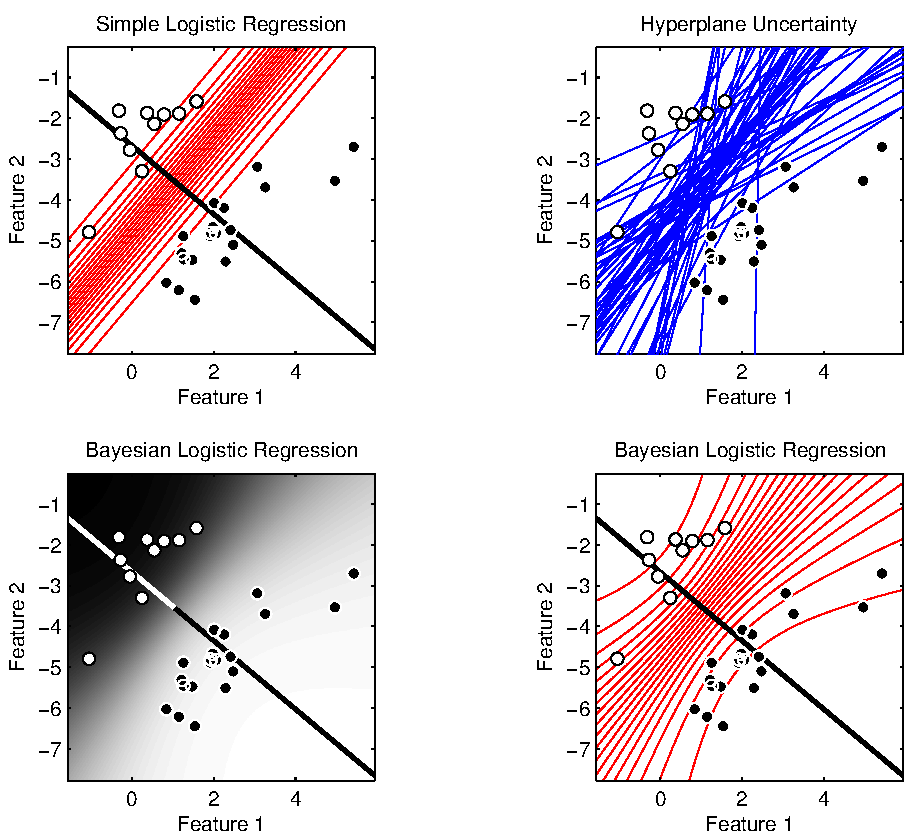
\includegraphics[width=\textwidth]{logistic_regr}
\end{columns}
\end{frame}

\begin{frame}
\frametitle{Woodbury matrix identity}
\begin{align*}
{\bf C}^{-1} = & \left(\sigma^{-2}{\bf X}{\bf X}^T + \Sigma_0^{-1}\right)^{-1}\\
             = & \Sigma_0 - \Sigma_0 {\bf X}({\bf I}\sigma^2 + {\bf X}^T \Sigma_0 {\bf X})^{-1} {\bf X} \Sigma_0
\end{align*}

\vspace{0.25cm}
\begin{tiny}
Wikipedia contributors, ``Woodbury matrix identity,'' Wikipedia, The Free Encyclopedia, \url{http://en.wikipedia.org/w/index.php?title=Woodbury\_matrix\_identity\&oldid=638370219} (accessed April 1, 2015).\par
\end{tiny}
\end{frame}

